
\documentclass[fontsize=10pt,twocolumn,letterpaper,abstracton]{scrartcl}
\typearea{20}
\usepackage[utf8]{inputenc}
\usepackage{hyperref}
\usepackage{graphicx}
\usepackage{amssymb}
\usepackage{amsmath}
\usepackage{wrapfig}
%\setlength{\droptitle}{-1in}
\usepackage{float}
\usepackage{titling}
\usepackage{comment} 

\pretitle{\noindent\centering\Large\bfseries}
\posttitle{\\}
\usepackage{caption}
\usepackage{multirow}
\usepackage{subcaption}
\usepackage{pgfplots}
\usepackage[margin=0.7in]{geometry}
\usepackage{color}
%\preauthor{\itshape}
%\postauthor{}
\predate{\itshape}
\postdate{}

\setlength{\columnsep}{2em}
\usepackage[small,compact,sc]{titlesec}

\title{Supervised Multi-Class Classification of Tweets}
\author{Zahan Malkani\\zahanm@stanford.edu \and Evelyn Gillie
  \\ egillie@stanford.edu}
\date{14 December, 2012}

\begin{document}
\maketitle

\begin{abstract}
  \textbf{We present a study of a variety of supervised learning methods used for the problem of Twitter tweet classification. This includes Support Vector Machines (SVM), Neural Networks (NN), Naive Bayes (NB), and Random Forests.  We evalutate these methods using their performance on two sources of labeled data: an `attitudes' dataset that classifies tweets with an attitude that the tweeter might have had when composing it, and a `topics' dataset that classifies tweets into one of a (limited-domain) topic set. We find that SVMs out-perform the others in accuracy and when used with feature selection have a reasonable runtime too.}
\end{abstract}

\section{Introduction}

The explosive growth of data being produced in the form of short text snippets has lead to an equally voracious growth in the methods used to analyze and decode these snippets. Machine learning plays an important role in enabling such analyses, since the vastness of these datasets vexes most hand-labeling attempts.

One of the more popular mechanisms producing this data is Twitter. The medium is notorious for confounding traditional text analysis methods, since the wealth of context that older natural language processing techniques depend on is simply missing in these tweets that are artificially confined to being 140 characters in length. Accordingly, selecting informative features to extract from the little context that we are given was a priority.

We explore a variety of supervised learning techniques to use in two classification tasks: 1), labelling tweets with an attitude from the \emph{speaker's} perspective (this is in contrast to most classification systems, that categorize tweets from the \emph{audience's} perspective, and usually just has two classes, \verb|positive| and \verb|negative|), and 2) labelling tweets based upon \emph{topics}, where we have a predefined set of topics that we are looking for.

We pursue modern approaches to classifying tweets, and explore their applications to real-world phenomena.

\section{Related Work}

Text classification is a well traversed area of machine learning, thanks to its potential for wide-reaching impact. \cite{textcat} and \cite{seqsampling} present good overviews of the methods used so far and their relative strengths and weaknesses. In \cite{textcat}, Yang and Liu go over the theory behind classifier methods such as Support Vector Machines, Neural Nets, k-Nearest Neighbor and Naive Bayes approaches. Their results do not offer much by way of quantitative outcomes of using these methods to classify short text snippets as we have. Lee makes some fascinating observations about how humans perform (long form) document classification in \cite{seqsampling}, providing a Bayesian model that fits how people seems to reason about this problem. His approach seems specific to the limited-domain topic classification problem though, that will be relevant for the second dataset in our paper.

In \cite{twsenti}, Agarwal et. al. discuss polarity features as inputs for supervised learning methods, specifically SVMs, in order to limit the feature space so that it can meaningfully be divided up by an SVM. These features, though we hadn't realized at the time, are similar in nature to the conditional frequency features that we trained our SVMs on eventually to capture the conditional probability of features corresponding to classes.

O'Conner et. al. provide very useful Twitter-specific tokenizers and emoticon analyzing algorithms in \cite{tweetmotif}, and the generalization of binary classification trees to the multi-class problem used by Lee and Oh in \cite{multitree} is the same as what we use for our multitree classification algorithm.

\section{Data}

\subsection{Data Collection}

In August, we started collected Twitter data using Twitter's streaming API on an Elastic Cloud Compute instance.
This collected around 55-60 tweets per second during peak hours, and 25-30 during non-peak hours. 

\subsubsection{Obama / Romney Dataset}

We selected a sample of 800 tweets from October 28$^{th}$ for Romney and 1300 tweets from November $4^{th}$ for Obama. We then had these tweets labeled with emotional attitudes on Amazon Mechanical Turk using Amazon certified categorizers, getting two categorizations for each tweet.

The emotional attitudes were chosen with consulation from a social data analytics startup, interested in a similar problem. Accordingly, we ended up with the set

\begin{verbatim}
{happy, mocking, funny, angry, sad,
hopeful, none / other}
\end{verbatim}

Workers agreed on the label on only $42.3\%$ of the samples. We manually reviewed a sample of the labels and found that for some tweets this is understandable, as what one person may construe as mockery another can readily define as anger, yet for a few tweets we would not have agreed with either. After consulting with the course staff we ultimately decided that the data was good enough to use as an experiment and left it at that. For the rest of the computations, if there are two labels and a classifier predicts one of them, we consider it correct.


\begin{table}
\centering
\begin{tabular}{ c | c }
Emotion & Percent of Dataset\\
\hline
Mocking & 0.45 \\
Funny & 0.28\\
Sad & 0.08\\
Angry & 0.03\\
Happy & 0.01\\
Hope & 0.01\\
None & 0.19\\
\end{tabular}
\caption{Distribution of Classes in Emotions Dataset}
\label{tb:emotdist}
\end{table}


\subsubsection{Topic Labeling Dataset}

Our second dataset uses a sample stream from August 6th, in which the Olympics are beginning, the Mars Rover had just landed, the Apple-Samsung lawsuit was in the press, and Obama was expectedly in the news.  Hence, tweets are labeled by their topic:

\begin{verbatim}
{obama, olympics, mars, apple, none}
\end{verbatim}

Overall, we collected around 3 million tweets, of which we labeled 100,000 using Mechanical Turk.  Of those 100,000, around 4,000 are labeled as being about any of the above topics.  

the topic distribution are shown in \ref{tb:topicdist}

\begin{table}[ht]
\centering
\begin{tabular}{ c | c }
Topic & Percent of Dataset\\
\hline
Olympics & 0.40 \\
Apple & 0.23\\
Mars & 0.22\\
Obama & 0.15\\
\end{tabular}
\caption{Distribution of Classes in Topical Dataset}
\label{tb:topicdist}
\end{table}


\subsection{Data Processing}

We take each tweet through a pipeline of steps. First, we lowercase the text to improve recall of unigram matching. Then we tokenize it with the Twitter-specific tokenizer from \cite{tweetmotif}, which preseves hashtags and emoticons. Then we perform Porter stemming on the words, again to improve recall of unigram matching. Then we construct singleton and bigram features for the tweet. The other features are discussed separately.

\subsubsection{Twitter Speech Features}

We wanted to more carefully consider the type of language used in the these text snippets. We considered a multitude of features that we chose ourselves, including

\begin{itemize}
\item Emoticons / Emoji
\item Punctuation (!!!!!)
\item Capitalization (LMAOOOO)
\item Dialogue (Retweets and @)
\item Negation
\item Sentence-level sentiment
\item Cursing
\end{itemize}

We were able to see some small improvement to SVM accuracy for certain classes through addition of these features, as can be seen in table \ref{tb:twspeech} (these tests were performed on a small, high-accuracy dataset).

\begin{table}[ht]
\centering
\begin{tabular}{c|c}
\begin{tabular}{c}
Bag-of-words \\
\begin{tabular}{cc}
emotion & accuracy \\
\hline 
angry  & .9533  \\
mocking  & 1 \\
happy  & .9828  \\
sad  & .9792  \\
hopeful  & .9811 \\
funny  & 1  \\
none  & .9719 \\
\end{tabular}
\end{tabular}

&

\begin{tabular}{c}
+ Twitter specific \\
\begin{tabular}{cc}
emotion & precision \\
\hline
angry  & .9659  \\
mocking  & .9699 \\
happy  & .9710 \\
sad  & 1 \\
hopeful  & .9709 \\
funny  & .9879 \\
none  & .9713 \\
\end{tabular}
\end{tabular}
\end{tabular}
\caption{Adding Twitter Speech Features to SVM Input}
\label{tb:twspeech}
\end{table}

It was disappointing to see that for most of the emotions our engineered features hurt performance, so we'd like to offer a special shout-out to the angry tweets for their user of upper-case and exclamation points.

\subsubsection{Class Distribution Features}

While exploring the performance of \verb|mocking| and \verb|angry|, we decided to analyze the normalized distribution of the sum of the weights by each token over an entire feature set, believing that this would enable us to see where some labels were nearly the winner only to just barely lose out to another label. More precisely,

Let
\begin{itemize}
\item $F = {f_{0}...f_{m}}$ be the vocabulary of features.
\item $S = {s_{0}...s_{n}}$ be the sample input such that $s_{i}$ is defined by its features $s_{i} = f_{0}f_{1}...f_{k}$ 
\item $L = {l_{0}...l_{n}}$ be the corresponding known labels be a multi-class vector.
\item $W$ be a $m \times n$ matrix such that $W_{i,j} = \sum_{s_{k} } I(f_{i} \epsilon s_{k}\ ^{\wedge}\ l_{k,j} = 1)$, namely W counts the co-occurences of features and labels.

\item for sample $s_{k}$, $v_{k}$ as 
$v_{k}=\sum_{f_{i}\epsilon s_{k}} W_{i,j}$
\end{itemize}

Upon analyzing the data we made the important realization that these vectors were strongly correlated with the labels, much more so than any element in isolation. We quickly tried these as feature vectors in our SVM framework and produced excellent results. We analyzed the literature for similar feature selection, and it seems Agarwal, et. al. introduce a similar polarity-prior term in \cite{twsenti}; our feature is an extension of this to the multi-class case.

Ultimately, we realized that these are precisely the conditional feature class counts that Naive Bayes exploits to good effect, but it provided a useful insight into the workings of SVMs.

\section{Algorithms}

%little theory for each
%then results in tabular format
%graphs? incremental improvements

\subsection{Feature Selection}
After stemming words and adding all words and bigrams to the feature set, our feature space is in the thousands.  With methods such as SVM or random forests, we need to trim down our feature set to get reasonable running times. We tried three feature selection methods:

Our first feature selector was a basic frequency pruner: features that did not occur frequently at all were thrown out (often, these were misspellings). %todo: stats

Our second feature selector was a mutual information feature selector.  Given a feature set F and class set C, the mutual information score is:\\
\begin{equation}
I(F;C) = \sum_{f,c} P(f,c)\log\frac{P(f,c)}{P(f)P(c)}
\end{equation}
Which translates to:\\

{ \centering{
$\frac{N_{11}}{N}ln(\frac{NN_{11}}{N_{1.}N{.1}}) + \frac{N_{01}}{N}ln(\frac{NN_{01}}{N_{0.}N{.1}}) + \frac{N_{10}}{N}ln(\frac{NN_{10}}{N_{1.}N{.0}}) + \frac{N_{00}}{N}ln(\frac{NN_{00}}{N_{0.}N{.0}})$\\
}
}

Where $N$ is the total number of tweets, $N_{11}$ is the number of tweets of the given class containing the given word, and $N_{01}$ is the number of tweets of any other class containing the given word.\\
Our third feature selector was $\chi^{2}$ feature selection:\\
\small
\begin{multline}
\centering
\frac{(N_{11}+ N_{10} + N_{01} + N_{00}) * (N_{11}N_{00} - N_{10}N_{01})^{2}}{(N_{11} + N_{01}) * (N_{10} + _{11}) *
(N_{10} + N_{00}) * (N_{01} + N_{00})}
\end{multline}
\normalsize

Mutual Information and $\chi^{2}$ feature selection is usually formulated in terms of binarry classification problems; we extend it to our multi-class problem by throwing out features whose maximum score with \emph{any} class is below some threshold.  That is, is a feature does not score highly with any class, we do not include it in our feature set.

\begin{table}[ht]
\centering
\begin{tabular}{ c | c | c | c | c }
Method & Threshold & features & runtime & accuracy\\
\hline
None & N/A & 6000 & 1m30s & 0.92\\
Frequency & 2 & 1093 & 25s & 0.93\\
MI & 0.01 & 1852 & 23s & 0.92\\
MI & 0.1 & 1716 & 20s & 0.93\\
MI & 0.2 & 1635 & 20s & 0.96\\
$\chi^{2}$ & 0.1 & 5989 & 20s & 0.87 \\
$\chi^{2}$ & 5.0 & 1814 & 25s & 0.91\\
$\chi^{2}$ & 20.0 & 184 & 10s & 0.89\\
\end{tabular}
\caption{Results of an SVM run using feature selection.  (Using 700 examples of the topics dataset)}
\label{tb:nb-inf}
\end{table}

Examples of high-scoring features for each feature selection method are shown in \ref{tb:featsel}

\begin{table*}[t]
\centering
\begin{tabular}{c|c}
\begin{tabular}{c}
Topical Dataset \\
\begin{tabular}{cc}
$\chi^{2}$ & Mutual Info \\
\hline 
presid & googl\\
billionair & ipod\\
money & \#teamusa\\
@marscurios & us \\
mar & planet\\
\#msl & iphon\\
money & 4s\\
iphon & @london2012\\
rover & basketball\\
olymp & planet \\
\end{tabular}
\end{tabular}

&

\begin{tabular}{c}
Obama \\
\begin{tabular}{cc}
$\chi^{2}$ & Mutual Info \\
\hline
ridicul (sad) & vote (hopeful)\\
lost (afraid) & lie (angry)\\
nate (happy) & elect (angry)\\
disturb (sad) & campaign (angry)\\
86\% (happy) & presid (angry) \\
lie (angry) & left (angry)\\
newspap (afraid) & tie (sad)\\
cnn (sad) & cnn (sad)\\
die (angry) & fight (hopeful)\\
random (afraid) & final (hopeful)\\
\end{tabular}
\end{tabular}
\end{tabular}
\caption{High-scoring features using feature selection}
\label{tb:featsel}
\end{table*}


\subsection{Naive Bayes}

The first learning algorithm that we tried was Naive Bayes.  Despite Naive Bayes' assumption of feature independence (an assumption which doesn't hold for natural language) it appears to perform resonably well on our datasets. The algorithm works by learning the conditional probability for each particular feature, conditioned on the label of the training example being processed. It then makes a prediction for an unlabeled point by calculating the posterior probability for each class and predicting the maximizing assignment.

\begin{equation} \label{eq:nb}
\underset{c}{\operatorname{argmax}} p(C=c) \prod_i^n p(F=f_i | C=c)
\end{equation}

The independence assupmtions made in NB (as can be seen in the second term of (\ref{eq:nb})), has the important side-effect of allowing a Naive Bayes classifier handle a large number of features with very little sacrifices in accuracy due to the curse of dimensionality that often effects other learning algorithms. This is very important for text classification, where often the feature space size dwarfs the other relevant dataset metrics.  

We see this particular trait serve Naive Bayes well, since it does rather well when using the simplest feature set: bernoulli prescence vectors, leading to what is often called the multivariate Bernoulli Naive Bayes classifier. The results are summarized in table \ref{tb:nb-accuracy}.

\begin{table}[H]
\centering
\begin{tabular}{ c c c }
Name & size & 10-fold accuracy \\
\hline
Romney dataset & 800 & 54\% \\
Obama dataset & 1300 &  41\% \\
Topics labeling & 40,000 & 78\% \\
\end{tabular}
\caption{Accuracy of Naive Bayes for each dataset}
\label{tb:nb-accuracy}
\end{table}

After running Naive Bayes, we looked at the conditional probabilities of each feature, and pulled out the most informative ones for each class as shown in table \ref{tb:nb-inf}.

\begin{table}[H]
\centering
\begin{tabular}{ c | c }
money & obama : olympi =    193.2 : 1.0\\
land,on  & mars : olympi =    144.4 : 1.0\\
rais  & obama : olympi =     90.5 : 1.0\\
@marscurios  & mars : apple  =     77.9 : 1.0\\
app  & apple : olympi =     60.0 : 1.0\\
what,you  & mars : olympi =     53.9 : 1.0\\
safe  & mars : olympi =     53.9 : 1.0\\
join  & obama : olympi =     50.3 : 1.0\\
land  & mars : olympi =     47.3 : 1.0\\
latest & mars : apple  =     45.5 : 1.0\\
busi  & obama : olympi =     45.0 : 1.0\\
youtub  & apple : olympi =     44.7 : 1.0\\
\end{tabular}
\caption{NB Most Informative Features}
\label{tb:nb-inf}
\end{table}

%TODO most important features - check after a NB run
One final note is that Naive Bayes is also a very fast classifier -- it handles a large feature space without a huge time cost.  Our implementation of NB classified all datasets in under 5 seconds.
\subsection{Neural Networks}
The next machine learning algorithm we applied was an Artifician Neural Network.  We used a Tahn layer, Softmax output multiclass neural network.  Using three hidden layers, we were able to achieve   86\% accuracy over the five-class topic dataset.  ANNs outperformed Naive Bayes, but with a huge time cost -- running 10-fold cross-validation in parallel over 700 examples took several minutes.

\begin{table}[H]
\centering
\begin{tabular}{ c | c | c | c}
Layers & Feat Sel & Threshold & Accuracy\\
\hline
2 & $\chi^{2}$ & 1.0 & 0.79\\
3 & None & N/A & 0.86\\
3 & $\chi^{2}$ & 1.0 & 0.87\\
3 & MI & 0.1 & 0.87\\
3 & MI & 0.2 & 0.86\\
3 & MI & 0.1 & 0.87\\
4 & $\chi^{2}$ & 0.1 & 0.83 \\
\end{tabular}
\caption{Neural Net Accuracies Over the Topical Dataset}
\label{tb:nb-inf}
\end{table}



\subsection{Support Vector Machines}

SVMs are widely known as an excellent learning model. We used an implementation from the Milk\cite{milk} library, and customized that as detailed below. 

\subsubsection{Multi-Class Classification}

In order to work with with multi-class classifications, we looked at two SVM models: one-vs-one and one-vs-rest.

\begin{table}[H]
\centering
\begin{tabular}{ c | c | c}
Dataset & mode & accuracy\\
\hline
Attitudes & one-vs-one & 0.57 \\
Attitudes & one-vs-rest & 0.59 \\
Topical & one-vs-one & 0.92 \\
Topical & one-vs-rest & 0.92 \\
\end{tabular}
\caption{SVM multiclass methods}
\label{tb:svm-method}
\end{table}

The one-vs-rest method appears to have slightly higher acuracy over the attitudes dataset, so we proceed with that.

We trained over the same features as in previous models (singletons, bigrams and twitter speech features), and to preprocess the data, we used feature selection to remove linearly dependant features, and also ran stepwise discriminant analysis (SDA). SDA functions by selecting the feature that is most correlated with preditions, removing its variance from the other features and then repeating the step to add more features. 


\textbf{Kernel}:
We experimented with two kernels: radial basis function and dot product.  For the radial basis function kernel, we performed a grid search over values of C from $2^{-2, -1, ... 3, 4}$ and $\sigma$ from -4 ... 4

\begin{table}[H]
\centering
\begin{tabular}{ c | c | c}
Dataset & mode & accuracy\\
\hline
Attitudes & RBF & 0.59 \\
Attitudes & Dot & 0.57 \\
Topical & RBF & 0.92 \\
Topical & Dot & 0.90 \\
\end{tabular}
\caption{A SVM Kernel Comparison}
\label{tb:nb-inf}
\end{table}

Again, the results are close, but the RBF kernel with grid search appears to outperform the dot product kernel.

Using the feature selection techniques outlined earlier and these optimal SVM settings, we were able to achieve a very high accuracy over the topical dataset.  Using $\chi^{2}$ feature selection, RBF kernel, and a one-vs-rest SVM classifier, we achieved 93\% 10-fold cross-validation accuracy over all 4000 examples.  

\begin{figure}[H]
\centering
    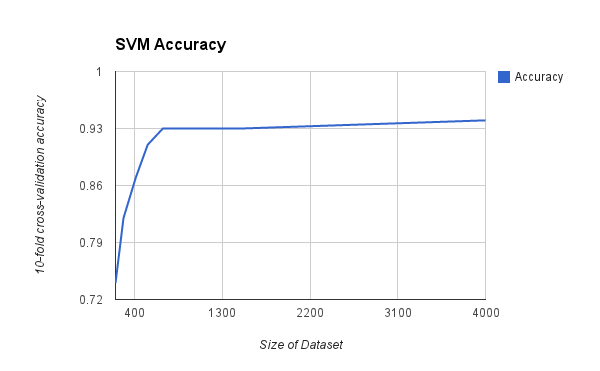
\includegraphics[scale=0.45]{svm_accuracy.png}
  \caption{SVM accuracy and Dataset Size (Topic Dataset)}
  \label{fig:svm_acc}
\end{figure}

\subsubsection{Class Distribution Features for Attitudes Dataset}

As discussed in the section on Class Distribution Features, we had a breakthrough on the attitudes dataset front, when we decided to use the class conditional probabilities of each feature to construct our SVM input space. We ended up settling on using just one input per class, that was the sum of the condition probabilities of each feature for that particular class, as seen in the training data.

Since these features were presumably highly seperable with the Radial Basis Function kernel, the SVM accuracy was greatly increased, and the runtime was brought down considerably. Running 10-fold cross validation on the datasets took no longer than 5 minutes. The results for running a one-vs-rest SVM using these inputs over the various attitudes datasets are presented in table \ref{tb:svm-cdf-accuracy}.

\begin{table}[H]
\centering
\begin{tabular}{ c c c }
Name & size & 10-fold accuracy \\
\hline
Romney dataset & 800 & 92\% \\
Obama dataset & 1300 &  90\% \\
Romney + Obama dataset & 2100 & 89\% \\
\end{tabular}
\caption{Accuracy of SVMs with Class Distribution Features}
\label{tb:svm-cdf-accuracy}
\end{table}

We would expect this technique to do better with increasing dataset size, but we suspect that internal variations in the datasets themselves (the Obama dataset had more uninformative tweets like \verb|LOOOL!!|) overpowered this overall effect.

\subsection{Random Forest}

We experimented with three random forest classifiers, using one-against-one, one-against-rest, ECOC (\cite{ECOC}, and multi-tree learners.  The multi-tree learner performed in the 70\% range on the topical dataset, using $\chi^{2}$ feature selection, and ECOC, one-against-one and one-against-rest yielded accuracies in the 90\% range.  We used stringent feature selection ($\chi$ $>$ 1.0) given the slowness of random forests.

\begin{table}[H]
\begin{tabular}{ c | c | c }
Learner & Training examples & Accuracy\\
\hline
ECOC & 700 & 0.92\\
Multi-tree & 700 & 0.72\\
one-against-rest & 700 & 0.81\\
one-against-one & 700 & 0.90\\
one-against-one & 1000 & 0.90\\
one-against-one & 2000 & 0.90\\
one-against-rest & 700 & 0.92\\
\end{tabular}
\caption{Neural Net Accuracies}
\label{tb:nb-inf}
\end{table}

Despite its high accuracy, we decided not to try ECOC with larger datasets due to its prohibitive slowness.

\section{Case Studies}

\subsection{Fans Reacting to an Underdog Comeback}

Now that we have a working model, we would like to evaluate it on real-world data. We collected approximately 80,000 tweets containg the keywords ``Saints'' or ``Seahawks'' between 1:00 pm and 4:00 pm on the day of a playoff game between the two teams . 

In this case, the 11-5 Saints were slated to dominate the game against the 7-9 Seahawks.  Surprisingly, the Seahawks won the game, causing a ripple of emotions to spread through the twitosphere. We captured that effect by analyzing the change in attitude distributions over twenty minute intervals.


\def\gametime{{"1:00", "1:20", "1:40", "2:00", "2:20", "2:40", "3:00", "3:20", "3:40"}}
\begin{figure}[H]
\begin{tikzpicture}[scale=0.95]
\begin{axis}[
    title = {Tweets Expressing Mockery},
    ylabel = Percentage,
    ymin =0.12, ymax = 0.40,
    xtick=data,
        xticklabel style= {rotate=45,anchor=north east},
        xticklabel={\pgfmathparse{\gametime[Mod(\tick,9)]}\pgfmathresult}]
     \addplot coordinates {
        (0,    0.160)
            (1,    0.184)
            (2,   0.195)
            (3,    0.195)
	    (4,    0.215)
	    (5,    0.218)
	    (6,    0.215)
	    (7,    0.213)
	    (8,    0.231)
        }; \addlegendentry{Both Teams}
     \addplot coordinates {
	    (0,    0.152)
            (1,    0.177)
            (2,   0.196)
            (3,    0.207)
	    (4,    0.240)
	    (5,    0.280)
	    (6,    0.258)
	    (7,    0.256)
	    (8,    0.283)
        }; \addlegendentry{Saints Only}
     \addplot coordinates {
	    (0,    0.207)
            (1,    0.242)
            (2,   0.267)
            (3,    0.222)
	    (4,    0.214)
	    (5,    0.202)
	    (6,    0.210)
	    (7,    0.204)
	    (8,    0.210)
        }; \addlegendentry{Seahawks Only}
\end{axis}
\end{tikzpicture}
\end{figure}

\begin{figure}
\begin{tikzpicture}[scale=0.95]
\begin{axis}[
	title = {Tweets Expressing Happiness},
	ylabel = Percentage,
	ymin =0.15, ymax = 0.55,
	xtick=data,
        xticklabel style= {rotate=45,anchor=north east},
        xticklabel={\pgfmathparse{\gametime[Mod(\tick,9)]}\pgfmathresult}]
     \addplot coordinates {
	    (0,    0.310)
            (1,    0.305)
            (2,   0.280)
            (3,    0.280)
	    (4,    0.292)
	    (5,    0.314)
	    (6,    0.268)
	    (7,    0.285)
	    (8,    0.273)
        }; \addlegendentry{Both Teams}
     \addplot coordinates {
	    (0,    0.328)
            (1,    0.351)
            (2,   0.329)
            (3,    0.286)
	    (4,    0.243)
	    (5,    0.226)
	    (6,    0.254)
	    (7,    0.224)
	    (8,    0.209)
        }; \addlegendentry{Saints Only}
     \addplot coordinates {
	    (0,    0.347)
            (1,    0.282)
            (2,   0.207)
            (3,    0.289)
	    (4,    0.335)
	    (5,    0.370)
	    (6,    0.289)
	    (7,    0.339)
	    (8,    0.326)
        }; \addlegendentry{Seahawks Only}
\end{axis}
\end{tikzpicture}
\end{figure}

We can see where the Saints took an early lead, at the end of the first quarter they were up 10-7. Over the next two hours, however, the Seahawks outscored the Saints 10-27. Then at the end of the game the Saints mounted a brilliant 16-10 rebound, but unfortuantely it was too little too late, and the Seahawks won the game.

Intuitively, these events align with the rise and fall of fans' emotions. We can even observe subtle differences, for example the difference at the 3:00 mark between \verb|mocking| and \verb|angry|, where Saints fans are angry at the Seahawks but not mocking them, while Saints fans are angry at the Saints and the Seahawks fans are mocking them.

We can see an interesting phenomenon with \verb|hopeful|, at the beginning of the game both sides are hopeful. Initially the Saints are expected to win and the Saints to lose, so when the Saints take an early lead the Seahawks lose their hope for an upset. When the tide is turned we can see a resurgence in hope. The truly interesting part is that henceforth both teams observe patterns related to when they scored, yet the overall amount of hope decreases steadily after the first half of the game, as fans are hopeful for the teams at the beginning of the game and then later pre-occupied with other emotions.

\begin{center}
\begin{tikzpicture}[scale=0.95]
\begin{axis}[
	title = {Tweets Expressing Hope},
	ylabel = Percentage,
	ymin =0.20, ymax = 0.45,
	xtick=data,
        xticklabel style= {rotate=45,anchor=north east},
        xticklabel={\pgfmathparse{\gametime[Mod(\tick,9)]}\pgfmathresult}]
     \addplot coordinates {
	    (0,    0.3458)
            (1,    0.3341)
            (2,   0.2882)
            (3,    0.2897)
	    (4,    0.3228)
	    (5,    0.3119)
	    (6,    0.2861)
	    (7,    0.2972)
	    (8,    0.2703)
        }; \addlegendentry{Both Teams}
     \addplot coordinates {
	    (0,    0.3832)
            (1,    0.3905)
            (2,   0.3264)
            (3,    0.2937)
	    (4,    0.3008)
	    (5,    0.2606)
	    (6,    0.2658)
	    (7,    0.2769)
	    (8,    0.2467)
        }; \addlegendentry{Saints Only}
     \addplot coordinates {
	    (0,    0.4005)
            (1,    0.3235)
            (2,   0.2605)
            (3,    0.3256)
	    (4,    0.3546)
	    (5,    0.3509)
	    (6,    0.3128)
	    (7,    0.3292)
	    (8,    0.2982)
        }; \addlegendentry{Seahawks Only}
\end{axis}
\end{tikzpicture}
\end{center}

\section{Conclusions}
Overall, SVM using a grid search over a Radial Basis Function Kernel outperformed Naive Bayes, neural nets, and random forests.  Random forest methods were able to come close to SVM accuracy, but were considerably slower.  Further, our feature selection methods were able to cut down dramatically on time without significant accuracy penalties.  \\
Even on the `attitudes' dataset, when used with our class distribution features, the SVM classifiers performed well, and seemed accurate enough to explore previously unseen tweets about a real-world event.

\section{Acknowledgements}

We would like to thank Austin Gibbons for his consultation on the project. We would like to thank Richard
Socher for his help in guiding the project. We would like to thank the InfoLab for lending us their computational and data resources.

\begin{thebibliography}{1}

\bibitem{textcat} Yiming Yang and Xin Liu. A Re-examination of Text Categorization Methods \url{http://www.inf.ufes.br/~claudine/courses/ct08/artigos/yang_sigir99.pdf}
\bibitem{seqsampling} Michael D. Lee. Fast Text Classification Using Sequential Sampling Processes \url{http://lvk.cs.msu.su/~bruzz/articles/classification/Fast%20Text%20Classification%20Using%20Sequential.pdf}
\bibitem{twsenti} Agarwal et al, Sentiment Analysis of Twitter Data, 2011.
\bibitem{tweetmotif} Brendan O'Connor, Michel Krieger, and David Ahn. TweetMotif: Exploratory Search and Topic Summarization for Twitter. ICWSM-2010.
\bibitem{milk} Milk. \url{http://luispedro.org/software/milk}
\bibitem{nltk} NLTK \url{http://nltk.org/}
\bibitem{multitree} Jin-Seon Lee and Il-Seok Oh. Binary Classification Trees for Multi-class Classification Problems \url{http://www.primaresearch.org/ICDAR2003/Papers/0141_503_lee_j.pdf}
\bibitem{ECOC} \url{http://www.cs.cmu.edu/afs/cs/project/jair/pub/volume2/dietterich95a.pdf}
\end{thebibliography}
\end{document}
